\chapter{前言}
\renewcommand{\baselinestretch}{10.0} %設定行距
\pagenumbering{arabic} %設定頁號阿拉伯數字
\setcounter{page}{1}  %設定頁數
\fontsize{14pt}{2.5pt}\sectionef
\section{研究動機}
高中職到大學現在所教的繪圖軟體都是老師在業界中所挑選出來的,不外乎最主要的軟體就是 Soidworks ,身為業界中中小企業最受歡迎的程式,只要是有畫 3D 繪圖的人都一定知道的,但在專題老師的介紹下,我們得知了不輸於 Solidworks 的繪圖軟體 Solid Edge 以及同公司旗下的限元素分析軟體 Femap 。 Solidworks 在台灣機械領域已經有個不可動搖的地位存在了,但我們必須讓這些不亞於 SW 的優良軟體浮出水面,讓更多的人知道不是只要學會 Solidworks 就行了!\\
我們將Solid Edge比Solidworks更有優勢的部分列出了以下幾點:
\begin{itemize}
\item 使用授權\\

\qquad 學生能在官網申請後,得到1000天的使用授權,且能用Solid Edge所有的軟體,無須因授權問題而使用非正版的軟體。\\

\item 分析軟體\\

\qquad Solid Edge內建Famap有限元素分析軟體,不用經過轉檔,建模完能直接分析。\\

\item 獨有技術\\

\qquad 同步建模與工程參照的讓建模時間大幅縮短,大幅減省時間與人力成本。\\

\item 可攜版本\\

\qquad 軟體不須透過網路取得權限,能直接將Solid Edge安裝在隨身硬碟上隨處使用。\\

\qquad 雖說能將Solid Edge安裝在USB上做使用,但不是說直接將Solid Edge的資料夾傳進隨身碟就好,需額外有圖裡的兩個登錄項目,讓沒有安裝過Solid Edge的主機登錄一堆細部項目,之後直接start-se2023就能使用了。\\

\qquad 但必須注意的是,這僅僅只是登錄檔,在stop時,並沒有附帶刪除登錄項目的功能,所以比較推薦在有還原卡的主機上做使用,而剛好全台學校的電腦主機幾乎都有還原卡,或者是路邊的網咖也行,就不需要在額外花時間載Solid Edge了,只需要帶個隨身碟,滑鼠點個兩下,就可以省去下載的時間。\\
\begin{figure}[hbt!]
\begin{center}
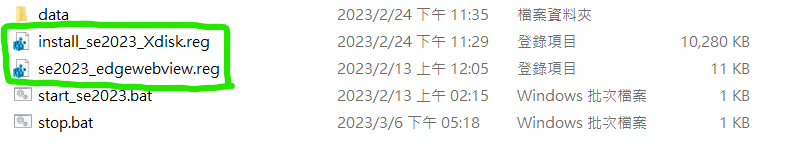
\includegraphics[width=10cm]{啟動檔}
\caption{\Large 可攜登錄檔}\label{0.1}
\end{center}
\end{figure}
\\
\section{Solid Edge 簡介}

\qquad Solid Edge 是一個完整的混合式 2D/3D CAD 系統,從零件、組裝、工程圖等研發工作流程一次完成。並搭載 Siemens 獨家 同步建模技術 ,能夠加速設計、更快的設計變更、提高匯入資料重用效率。\\

\qquad 同步建模技術結合了速度和靈活性,直接建模,控制精確的尺寸驅動設計(功能和同步解決相關的參數)。參數的關係,可直接應用於固體功能,而不必依賴於二維草圖幾何關係和共同參數自動應用。該建模過程是表示要爭取一定的 CAD 設計活動高達100倍的速度。\\

\qquad 不像其他直接建模系統,它不是典型的帶動歷史的建模方法,而不是提供參數化尺寸驅動的建模幾何通過同步,參數和使用規則的決策引擎,讓用戶使用不可預測的變化。這個對象驅動的編輯模式是被稱為對象操作界面,它強調一個用戶界面,提供直接操縱的對象( DMUI )。\\

\qquad 2007年, SIEMENS (西門子股份有限公司)工業自動化部門收購了 UGS 公司,後將 UGS 的公司更名為 Siemens PLM Software 。 \\

\item Solid Edge 有限元分析 (FEA)\\

\qquad 通過內建的有限元分析 (FEA) 工具,設計工程師可以在 Solid Edge 環境中通過數字方式驗證零件和組立件設計。Femap 有限元建模和 NX Nastran 求解器技術業已成熟,Solid Edge 分析在此基礎上,使實體原型需求顯著下降,從而降低材質和測試成本,縮短設計時間。\\

\item Solid Edge FloEFD 流體分析 (CFD)\\

\qquad FloEFD for Solid Edge 是一款可完全嵌入 Solid Edge 內的前端載入計算流體力學 (CFD) 分析工具。通過內嵌式 CFD 分析工具,輕鬆、快速且準確地進行流體流動和熱傳導分析。與其他 CFD 工具相比較, 該工具可將解決方案的整體時間縮短多達百分之65-百分之75 。\\

■ 基本模組 ■ 電子散熱模組 ■ 暖通空調模組\\
■ LED 模組 ■ 進階應用模組 ■ 電路模組\\

\section{Femap 簡介}

\qquad Femap 是一高級工程模擬應用程序,用於建立、編輯和導入 / 重用複雜產品或系統的以網格為中心的有限元分析模型。您可使用 Femap 對零件、組件或系統進行建模,並確定給定操作環境的行為響應。\\

\qquad Femap 還提供強大的數據驅動和圖形結果可視化和評估。您可將 Femap 與各種 CAD 系統和有限元分析求解器(包括業界領先的 NX Nastran 應用程序)相結合,提供全面的計算機輔助工程分析解決方案,幫助確保產品在實際環境中按設計運行。 \\

\end{itemize}

\renewcommand{\baselinestretch}{0.5} %設定行距